%!TEX root = met-top-spaces.tex
\stepcounter{lecture}
\setcounter{lecture}{4}
\sektion{Compactness}

\subsection{Basic notions} % (fold)
\label{sub:compact:basic_notions}

\begin{definition}
	Let $(X,\tau)$ be a topological space. An \emph{open cover of $X$} is a collection of open subsets $\cover=\{U_\gamma:\gamma\in\Gamma\}$ such that $X=\bigcup_{\gamma\in\Gamma} U_\gamma$.
	
	If $Y\subset X$, then an open cover of $Y$ is a collection of open subsets in $X$ $\cover=\{U_\gamma:\gamma\in\Gamma\}$ such that $Y\subset\bigcup_{\gamma\in\Gamma} U_\gamma$.
\end{definition}

\vspace{3pt}

\begin{remark}
	Such an open cover of $Y$ provides a base of open sets $\cover = \{U_\gamma \cap Y: \gamma\in\Gamma\}$ for $Y$ with the subspace topology, and conversely.
\end{remark}

\vspace{-3pt}

\begin{definition}
	A \emph{subcover} of an open cover $\cover$ is a subcollection $\subcover \subseteq \cover$ which is still an open cover of $Y$.
\end{definition}

\begin{example}
	The intervals $I_n=(-n,n)$, where $n=1,2,\ldots$, form an open cover of $\R$, and $I_{n^2}$ is a proper subcover. The intervals $J_n = (n-1,n+1)$, where $n\iZ$, form an open cover of $\R$ with no proper subcover.
\end{example}

\begin{definition}
	A topological space $(X,\tau)$ is \emph{compact} if every open cover has a finite subcover.
\end{definition}

\begin{examples}
	In this sense, $\R$ is not compact, as the open covers described above have no finite subcovers. Any finite topological space is compact, as is any set with the indiscrete topology (the only open subsets of $X$ being $\emptyset$ and $X$), or with the cofinite topology.
\end{examples}

With this definition, compactness is a topological property.

\begin{lemma}
	Let $(X,\tau)$ be a topological space with $Y\subset X$. Then $Y$ is compact in the subspace topology if and only if every open cover $\{U_\gamma\}$ of $Y$ has a finite subcover.
\end{lemma}

\begin{proof}
	First let $\{U_\gamma:\gamma \in \Gamma\}$ be an open cover of $Y$, then $Y = \bigcup_{\gamma\in\Gamma} (U_\gamma \cap Y)$, where the $U_\gamma \cap Y$ are open in $Y$. Since $Y$ is compact, there exist $\gamma_1,\ldots,\gamma_n \in \Gamma$ such that $Y=\bigcup_{i=1}^n (U_{\gamma_i}\cap Y)$, and then $\{U_{\gamma_i}: i=1,\ldots,n\}$ covers $Y$.

	Now the converse. Suppose $Y=\bigcup_{\gamma\in\Gamma} V_\gamma$, where the $V_\gamma$ are open in $Y$. Write $V_\gamma = U_\gamma \cap Y$, where the $U_\gamma$ are open in $X$ and form an open cover of $Y$. Then there exist $\gamma_1,\ldots,\gamma_n \in \Gamma$ such that $Y \subseteq \bigcup_{i=1}^n U_{\gamma_i}$, and hence $Y=\bigcup_{i=1}^n V_{\gamma_i}$.
\end{proof}

\begin{example}
	The open interval $(0,1)$ is not compact: consider the open cover by intervals $(1/n,1-1/n$ for $n=3,4,\ldots$.
\end{example}

	\pagebreak

\begin{theorem}
	[Heine-Borel theorem] The closed interval $[a,b] \subset $ is compact.
\end{theorem}

\begin{proof}
	Let $[a,b] \subset \bigcup_{\gamma\in\Gamma} U_\gamma$, for $U_\gamma$ open in $\R$. Then set
	\begin{equation*}
		K = \left\{x\in[a,b]: \text{$[a,x]$ is contained in a finite union of the $U_\gamma$}\right\}.
	\end{equation*}
	Clearly $a\in K$, so $K\neq \emptyset$. Let $r=\sup K$. Then $r\in[a,b]$, and so $r\in U_{\gamma_1}$ for some $\gamma_1 \in \Gamma$. Since $U_{\gamma_1}$ is open, there exists $\delta>0$ such that $[r-\delta,r+\delta] \subseteq U_{\gamma_1}$.

	\begin{center}
		\begin{tikzpicture}[xscale=2,scale=3]
			
			\draw (-0.2,0) -- (1.2,0);
			\draw [very thick, |-|] (0,0) node [below=5pt] {$0$} -- (1,0) node [below=5pt] {$1$};

			\draw [thick, |-|] (0,0) -- (0.6,0) node [below=7.2pt] {\small{$r$}};

			\draw [thick, |-|] (0.45,0) node [below=5pt] {\small{$r-\delta$}} -- (0.75,0) node [below=5pt] {\small{$r+\delta$}};

			\draw [ultra thick, (-] (0.4,0) -- (0.41,0);
			\draw [ultra thick, -)] (0.94,0) -- (0.95,0);

			\bigarrow [dashed, <->] (0.4,0.2) -- (0.95,0.2);
			\bigarrow [dashed] (0.95,0.2) -- (0.4,0.2);
			\draw (0.675,0.2) node [above] {$U_{\gamma_1}$};

		\end{tikzpicture}
	\end{center}

	By the definition of $r$, there exists $c\in[r-\delta,r]$ such that $[a,c]$ is contained in a finite union of the $U_\gamma$. Hence, the same is true for $[a,r+\delta] \cap [a,b]$ (we just need to include $U_{\gamma_1}$ also). But this contradicts $r$ as an upper bound, unless $r=b$, in which case, the above argument tells us that $[a,b]$ is covered by finitely many of the $U_\gamma$. (There exists $c\in[b-\delta,b]$ such that $[a,c]$ is covered by finitely many $U_\gamma$, and include $U_{\gamma_1}$ also.)
	
	Thus $[a,b]$ is compact.
\end{proof}

\begin{proposition}
	A continuous image of a compact set is compact. \label{prop:cts-compact}
\end{proposition}

\begin{proof}
	Suppose $f:(X,\tau)\to(Y,\sigma)$ is a continuous map of topological spaces, and $K\subseteq X$ is compact. Then we wish to show that $f(K)$ is compact.

	Suppose $f(K)\subseteq\bigcup_{\gamma\in\Gamma} U_\gamma$, with $U_\gamma$ open in $Y$. Since $f$ is continuous, $K\subset\bigcup_{\gamma\in\Gamma} f^{-1}(U_\gamma)$, and each $f^{-1}(U_\gamma)$ is open in $X$. Since $K$ is compact, there exist $\gamma_1,\ldots,\gamma_n \in \Gamma$ such that $K\subseteq\bigcup_{i=1}^n f^{-1}(U_{\gamma_i})$, and hence $f(K)\subseteq\bigcup_{i=1}^n U_{\gamma_i}$. %
\end{proof}

\begin{proposition}
	A closed subset of a compact topological space $X$ is compact. \label{prop:closed-compact}
\end{proposition}

\begin{proof}
	Let $X$ be a compact topological space, and $K\subseteq X$ be closed. If $K=\emptyset$ then this is trivial, so assume not. Suppose $K\subseteq \bigcup_{\gamma\in\Gamma} U_\gamma$, where the $U_\gamma$ are open in $X$. Then $X=(X\backslash K)\cup\left( \bigcup_{\gamma\in\Gamma}U_\gamma \right)$, where $X\backslash K$ is also open. Since $X$ is compact, there is a finite subcover, and hence there exists $\gamma_1,\ldots,\gamma_n \in \Gamma$ such that $X=(X\backslash K) \cup \left( \bigcup_{i=1}^n U_{\gamma_i} \right)$. Thus $K\subseteq \bigcup_{i=1}^n U_{\gamma_i}$.
\end{proof}

\begin{proposition}
	Every compact subset of a Hausdorff topological space is closed. \label{prop:compact-hausdorff-closed}
\end{proposition}

\begin{proof}
	Let $X$ be a Hausdorff topological space, and $K \subseteq X$ be compact. If $K=X$, this is trivial, so suppose not. Then we show that $X\backslash K$ is open. 


	Given $x\in X\backslash K$, for any $y\in K$< there are disjoint open sets with $U_y \ni x$ and $V_y \ni y$. Now $\{V_u: y\in K\}$ is an open cover of $K$. Since $K$ is compact, there exist $y_1,\ldots,y_n \in K$ such that $K \subseteq \bigcup_{i=1}^n V_{y_i}$. Then $U=\bigcap_{i=1}^n U_{y_i}$ is an open neighbourhood of $x$ with $U\cap K = \emptyset$, so $U\subseteq X\backslash K$, as required.
\end{proof}

	\pagebreak

\begin{corollary}
	A set $X\subset\R$ is compact if and only if it is closed and bounded. \label{cor:comp-iff-clsed-bded}
\end{corollary}

\begin{proof}
	If $X\subset\R$ is compact, then proposition~\ref{prop:compact-hausdorff-closed} tells us that $X$ is closed (since $\R$ is Hausdorff). It is also bounded: if not, the open sets $U_m=\left\{x\iR: \left\vert x \right\vert<m\right\}$ form an open cover of $X$ with no finite subcover, contradiction.

	Now the converse. Suppose $X\subset\R$ is closed and bounded. Then there is $M$ such that $\left\vert x \right\vert\leq M$ for all $x\in X$ and so $X\subset[-M,M]$. Since $X$ is closed, $\R\backslash X$ is open, and so $(\R\backslash X)\cap[-M,M]$ is open in $[-M,M]$, and $X$ is closed in $[-M,M]$. Then by Heine-Borel, $X$ is compact, and so $X$ is compact by proposition~\ref{prop:closed-compact}.
\end{proof}

\vspace{3pt}

\begin{remark}
	We'll see later that the product of finitely many compact spaces is compact, and hence $\left[ -M,M \right]^n$ is a compact subset of $\Rn$. So a set $X\subset\Rn$ is bounded if and only if $\exists\,M$ such that $X\subset\left[ -M,M \right]^n$. From the proof of corollary~\ref{cor:comp-iff-clsed-bded}, this extends immediately to show that:
\end{remark}

\begin{corollary}
	A subset $X\subset\Rn$ is compact if and only if it is closed and bounded. \label{cor:compact-clsd-bded}
\end{corollary}

\vspace{-9pt}

\begin{examples}
\mbox{}
\begin{enumerate}
	\shortskip
	\item Combining this with theorem~\ref{thm:cnncted-R-interval}, the only connected compact subsets of $\R$ are closed intervals $[a,b]$.
	\item The Cantor set $C\subset[0,1]$ was defined by $C=\bigcap_{n\geq 0} I_n$, where $[0,1]=I_0\supset I_1\supset I_2\supset \cdots$, and $I_n$ was the diagonal union of $2^n$ closed intervals. Thus each $I_n$ is closed, and so $C$ is closed and bounded. Thus $C$ is compact.
\end{enumerate}
\end{examples}

We can now combine propositions~\ref{prop:cts-compact}, \ref{prop:closed-compact} and~\ref{prop:compact-hausdorff-closed} into a particular useful result:

\begin{corollary}
	Suppose $X$ is a compact space, $Y$ is a Hausdorff space, and $f:X\to Y$ is a continuous bijection. Then $f$ is a homeomorphism. \label{cor:quot-result}
\end{corollary}

\begin{proof}
	Let $g:Y\to X$ be the inverse map $f^{-1}$. We must show that this is continuous. Let $F\subseteq X$ be closed.

	Since $X$ is compact, proposition~\ref{prop:closed-compact} tells us that $F$ is compact. Since $f$ is continuous, proposition~\ref{prop:cts-compact} tells us that $g^{-1}(F) = f(F)$ is compact. Finally, $Y$ is Hausdorff, so by proposition~\ref{prop:compact-hausdorff-closed}, $g^{-1}(F)$ is closed in $Y$. Hence $g$ is continuous.
\end{proof}

This result is particularly useful in identifying quotient spaces.

\begin{example}
	Define $\sim$ on $\R$ by $x\sim y$ if and only if $x-y \iZ$, and let $\bb{T} = \{z\iC: \left\vert z \right\vert=1\}$ be the unit circle (with the subspace topology from $\C$). Now consider the map given by
	\begin{equation*}
		\fullfunction{f}{\R}{\bb{T}}{x}{\exp(2\pi ix)}
	\end{equation*}
	This is continuous and induces a bijection $\fbar:\R/\sim\, \to \bb{T}$, which, by definition of the quotient topology, is also continuous. (See our remark about quotient topologies on page~\pageref{rmk:quot-topologies}.)

	But the quotient map $q:\R\to\R/\sim$ restricts to a continuous surjection $[0,1]\to\R/\sim$. Since $[0,1]$ is compact, proposition~\ref{prop:cts-compact} tells us that $\R/\sim$ is compact. Then $\bb{T}$ is Hausdorff, and so corollary~\ref{cor:quot-result} tells us that $\fbar$ is a homeomorphism.

		\pagebreak

	In a similar way, we can show that the two-dimensional torus $\R^2/\Z^2$ is homeomorphic both the product space $S^{\,1} \times S^{\,1}$ (where $S^{\,1}$ is the unit circle), and to the embedded torus $X\subset \R^3$, consisting of points $((2+\cos\phi) \cos\theta, (2+\cos\phi) \sin\theta, \sin\phi)$, where $0\leq \theta,\phi < 2\pi$.

	\newcommand{\biggarrow}{\draw [decoration={markings,mark=at position 1 with {\arrow[scale=2]{>>}}},
    		   postaction={decorate},
    		   shorten >=0.4pt]}

	\vspace{3pt}

	\begin{center}
		\begin{minipage}{0.5\textwidth}
			\centering
			\begin{tikzpicture}[scale=2.25]
				
				\draw (0,0) rectangle (1,1);

				\foreach \s in {0,1} {
					\bigarrow (0,\s) -- (0.5,\s);
					\biggarrow (\s,0) -- (\s,0.6);
				}	

			\end{tikzpicture}
		\end{minipage}
		\begin{minipage}{0.45\textwidth}
			\centering
			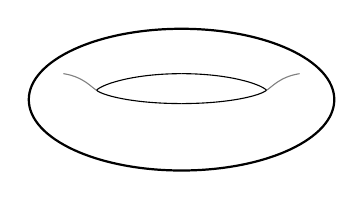
\begin{tikzpicture}[scale=0.2, yscale=0.5]

				\draw [thick] (0,0) circle (9.7 and 9);

				\draw (0,3.3) .. controls (3,3.3) and (5,2) .. (5.4,1.2);
				\draw (0,-0.5) .. controls (3,-0.5) and (5,0.5) .. (5.4,1.2);

				\draw (0,3.3) .. controls (-3,3.3) and (-5,2) .. (-5.4,1.2);
				\draw (0,-0.5) .. controls (-3,-0.5) and (-5,0.5) .. (-5.4,1.2);

				\draw [thin, gray] (5.4,1.2) .. controls (5.7,1.5) and (6.2,2.9) .. (7.5,3.3);
				\draw [thin, gray] (-5.4,1.2) .. controls (-5.7,1.5) and (-6.2,2.9) .. (-7.5,3.3);
			\end{tikzpicture}
		\end{minipage}
	\end{center}

	\begin{center}
		\begin{minipage}{0.5\textwidth}
			\centering
			the 2-D torus $\R^2/\Z^2$
		\end{minipage}
		\begin{minipage}{0.45\textwidth}
			\centering
			the embedded torus $X\subseteq \R^3$
		\end{minipage}
	\end{center}

	In \emph{Analysis I}, you learnt that continuous real-valued functions on $[a,b]\subseteq\R$ are bounded and attain their bounds. Here, we are using the compactness of $[a,b]$. This statement is still true, for instance, for continuous real-value functions on the Cantor set.
\end{example}

\begin{proposition}
	Continuous real-valued functions on a compact space $X$ are bounded and attain their bounds.
\end{proposition}

\begin{proof}
	Suppose $X$ is compact and $f:X\to\R$ is continuous. Then proposition~\ref{prop:cts-compact} tells us that $f(X)$ is compact, and so corollary~\ref{cor:compact-clsd-bded} tells us that $f(X)$ is bounded and closed.

	Since $f(X)$ is closed, it contains all of its accumulation points. But $\sup f(X)$ and $\inf f(X)$ (which exist because $f(X)$ is bounded) are accumilation points for $f(X)$, so $\sup f(X), \inf f(X) \in f(X)$, which gives the desire result.
\end{proof}

\begin{theorem}
	The product of two compact spaces is compact.
\end{theorem}

\begin{proof}
	Suppose $X$ and $Y$ are compact and that $X\times Y=\bigcup_{\gamma\in\Gamma} U_\gamma$, where the $U_\gamma$ are open in $X\times Y$.

	By the definition of the product topology, each $U_\gamma$ is the union of ``basic open sets'' of the form $V \times W$, where $V$ is open in $X$ and $W$ is open in $Y$. Thus
	\begin{equation*}
		X\times Y=\bigcup_{\delta\in\Delta} V_\delta \times W_\delta,
	\end{equation*}
	with $V_\delta$ open in $X$, $W_\delta$ open in $Y$ and $V_\delta \times W_\delta$ a subset of some $U_\gamma$.

	Now let $x\in X$, and then we have
	\begin{equation*}
		\{x\} \times Y \subseteq \bigcup_{\delta\in\Delta} V_\delta \times W_\delta,
	\end{equation*}
	such that $x\in V_\delta$.

	Now, since $Y$ is compact, there exist $\delta_1,\ldots,\delta_m$ such that $Y=\bigcup_{i=1}^m W_{\delta_i}$.

	Then let $V_x = \bigcap_{i=1}^n V_{\delta_i}$ be an open neighbourhood of $x$ such that $V_x \times Y \subseteq \bigcap_{i=1}^n V_{\delta_i} \times W_{\delta_i}$. The $V_x$ obtained in this way form an open cover of $X$, and so there exist $x_1,\ldots,x_n$ such that $X = \bigcup_{j=1}^n V_{x_j}$.

	Now $X\times Y=\bigcup_{j=1}^n V_{x_j} \times Y$ and each $V_{x_j} \times Y$ has a finite cover by $V_\delta\times W_\delta$'s. Thus $X\times Y$ has a finite cover by such sets. Since each $V_\delta\times W_\delta$ is a subset of some $U_\gamma$, $X\times Y$ has a finite cover by $U_\gamma$'s. Thus $X\times Y$ is compact.
\end{proof}

	\pagebreak

\begin{remarks}
	Given topological spaces $X,Y,Z$, the product $X\times Y \times Z$ is homeomorphic to $X \times \left( Y\times Z \right)$ under the obvious map (since a base for the topology of $X\times Y \times Z$ consists of subsets $U\times V \times W$, and a base for the topology of $X \times \left( Y\times Z \right)$ consists of subsets $U\times \left( V\times W \right)$, for $U$ open in $X$, $V$ open in $Y$ and $W$ open in $Z$. Hence open sets in $X \times Y \times Z$ correspond to open sets in $X\times \left( Y\times Z \right)$.) By induction, the above theorem implies that the product of finitely many compact spaces is compact.

	Now applying corollary~\ref{cor:compact-clsd-bded}, we see that $\left[ -M,M \right]^n$ is a compact subset of $\Rn$. The proof of the same corollary may be extended to show that $X\subseteq \Rn$ is compact if and only if $X$ is closed and bounded.
\end{remarks}

\begin{proposition}
	Let $X$ be a compact metric space, $Y$ a metric space and $f:X \to Y$ a continuous map. Then $f$ is \emph{uniformly continuous}; that is, given $\epsilon>0$, there exists $\delta>0$ such that for all $x,y\in X$, $d_X(x,y) < \delta$ implies $d_Y(f(x),f(y))<\epsilon$.
\end{proposition}

\begin{proof}
	Since $f$ is continuous, for all $x\in X$, there exists $\delta_x$ such that $d_X(x,y) < 2\delta_x$ implies $d_Y(f(x),f(y)) < \epsilon/2$. Now let
	\begin{equation*}
		U_x = \left\{y: d_X(x,y) < \delta_x \right\}.
	\end{equation*}
	The $U_x$ form an open cover of $X$, and so there exist $x_1,\ldots,x_n$ such that $X=\bigcup_{i=1}^n U_{x_i}$. Let $\delta=\min\{\delta_{x_i}\}$.

	Suppose now $d_X(y,z) < \delta$; since the $U_{x_i}$ form a cover, we can find $x_i$ such that $d(y,x_i) < \delta_{x_i}$. Since $d_X(y,z) < \delta<\delta_{x_i}$, we deduce that $d_X(z,x_i) < \delta + \delta_i < 2\delta_i$ (from the triangle inequality). Thus
	\begin{equation*}
		d_Y(f(y),f(z))
		< d_Y(f(y),f(x_i)) + d_Y(f(x_i),f(z))
		< \epsilon/2 + \epsilon/2
		= \epsilon. \qedhere
	\end{equation*}
\end{proof}

% subsection compact:basic_notions (end)

\subsection{Sequential compactness} % (fold)
\label{sub:sequential_compactness}

\begin{definition}
	A topological space is \emph{sequentially compact} if every sequence in $X$ has a convergent subsequence.
\end{definition}

\vspace{3pt}

\begin{remark}
	For general topological spaces, the property of compactness and sequential compactness are independent; neither implies the other.
\end{remark}

\begin{proposition}
	Any compact metric space is sequentially compact.
\end{proposition}

\vspace{-6pt}

Notice that this can be reduced to the Bolzano-Weierstrass theorem: namely, that any closed bounded subset of $\Rn$ is sequentially compact.

\begin{proof}
	Suppose $(X,d)$ is a metric space and $(x_n)_{n=1}^\infty$ is a sequence in $X$ with no convergent subsequence (in particular, there are infinitely many distinct $x_n$). We claim that for all $x\in X$, there exists $\delta>0$ such that $d(x,x_n) < \delta$ for at most finitely many $n$.

	If not, then there exists $x\in X$ such that for all $m>0$ in $\N$, $d(x,x_n)<1/m$ for infinitely many $n$, and hence there is a subsequence of $(x_n)$ converging to $x$, which is a contradiction.

	For each $x$, pick such a $\delta=\delta(x)$ and let $U_x = \{y:d(x,y) < \delta\}$. Each $U_x$ contains $x_n$ for only finitely many $n$. But $\{U_x:x\in X\}$ is an open cover for $X$, for which no finite subcover can exist. Hence $X$ is not compact.
\end{proof}

\begin{exercise}
	Show directly that if $X\subseteq\Rn$ is sequentially compact, then it is bounded, closed and hence compact. (Bounded, since otherwise we can find $(x_n)$ such that $d(x_n,x_0) > n$, which implies that there is no convergent subsequence.)
\end{exercise}

More generally, we have:

\begin{theorem}
	Suppose $(X,d)$ is a sequentially compact metric space. Then
	\begin{enumerate}
		\shortskip
		\item Given any $\epsilon>0$, there exists $x_1,\ldots,x_n$ such that $X=\bigcup_{i=1}^n B(x_i,\epsilon)$;
		\item Given any open cover $\cover$ of $X$, there exists $\epsilon>0$ such that for all $x\in X$, $B(x,\epsilon)$ is contained in some element $U$ of $\cover$.
		\item $(X,d)$ is compact.
	\end{enumerate}
\end{theorem}

\begin{proof}
\mbox{}
\begin{enumerate}
	\item Suppose not. Then by induction, we can construct a sequence $(x_n)$ in $X$ such that $d(x_m,x_n) \geq \epsilon$ for all $m\neq n$. Clearly such a sequence has no convergent subsequence, since no subsequence can satisfy the Cauchy condition. Contradiction.

	\item Suppose not. Then there exists an open cover $\cover$ of $X$ such that for all $n$, there exists $x_n\in X$ such that $B(x_n,1/n) \not \subseteq U$, for all $U \in \cover$. But $(x_n)$ has a subsequence $(x_{n(r)})$ tending to $x\in X$. So let $x\in U_0$, for some $U_0 \in \cover$. Since $U_0$ is open, there exists $m>0$ such that $B(x,2/m) \subseteq U_0$.

	\begin{center}
		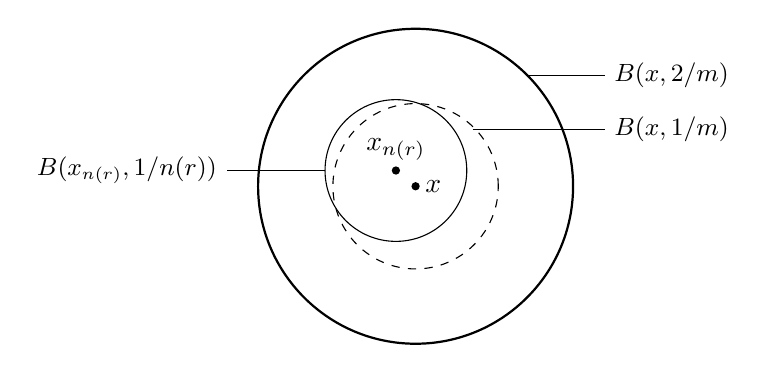
\begin{tikzpicture}

			\foreach \s/\t in {0/0, -0.25/0.2} {\fill [black] (\s,\t) circle (1.5pt);}

			\draw (0,0) node [right] {$x$};
			\draw (-0.25,0.2) node [above] {$x_{n(r)}$};

			\draw [thick] (0,0) circle (2);
			\draw [dashed] (0,0) circle (1.05);

			\draw (-0.25,0.2) circle (0.9);

			\draw (1.41,1.41) -- (2.4,1.41) node [right] {\small{$B(x,2/m)$}};
			\draw (0.725,0.725) -- (2.4,0.725) node [right] {\small{$B(x,1/m)$}};

			\draw (-1.15,0.2) -- (-2.4,0.2) node [left] {\small{$B(x_{n(r)},1/n(r))$}};
		\end{tikzpicture}
	\end{center}

	Now, there exists $N$ such that $x_{n(r)} \in B(x,1/m)$ for all $r\geq N$. Additionally, if $n(r)>m$, and $y\in B(x_{n(r)},1/n(r))$, then $d(x,y) \leq d(x,x_{n(r)}) + d(x_{n(r)},y) < 2/m$. So for such $n(r)$, $B(x_{n(r)}, 1/n(r)) \subseteq B(x,2/m) \subseteq U_0$. Contradiction.
	
	\item Let $\cover{U}$ be an open cover of $X$. Choose $\epsilon>0$ as in (ii). For this $\epsilon$, using (i), there exists $x_1,\ldots,x_n \in X$ such that $X=\bigcup_{i=1}^n B(x_i,\epsilon)$. For each $i$, $B(x_i,\epsilon) \subseteq U_i$ for some $U_i \in \cover$, by (ii). Thus $X=\bigcup_{i=1}^n U_i$, and $X$ is compact. \qedhere
\end{enumerate}
\end{proof}

% subsection sequential_compactness (end)